\chapter{Penalized multivariate regression}
\minitoc


\section{Ridge regression}
In the case where $X^\top X$ is singular (resp. has eigenvalues close to zero), the least squares estimate cannot be computed (resp. is not robust). A common approach to control the estimator variance is to solve the surrogate Ridge regression problem:
\[
\widehat \param^{\mathrm{ridge}}_{n,\lambda}\in  \argmin_{\param\in\rset^d}  \left\{\frac{1}{n}\|Y - X\param\|_2^2 + \lambda\|\param\|_2^2\right\}\eqsp,
\]
where $\lambda>0$. 
\begin{remark}
The matrix $n^{-1}X^\top X + \lambda  I_n$ is definite positive for all $\lambda>0$ as for all $u\in\rset^d$,
\[
u^\top (n^{-1}X^\top X + \lambda I_n)u = n^{-1}\|Xu\|_2^2 + \lambda  \|u\|_2^2\eqsp,
\]
which is positive for all $u\neq 0$. This remark allows to obtain the following result.
\end{remark}

\begin{shaded}
\begin{proposition}
\label{prop:least:squares:ridge}
The unique solution to the Ridge regression problem is given by
\[
\widehat \param^{\mathrm{ridge}}_{n,\lambda} = \frac{1}{n}\left(\frac{1}{n}X^\top X + \lambda I_n\right)^{-1}X^\top Y\eqsp.
\] 
In the well-specified setting, this estimator is biased and satisfies 
\begin{align*}
\bE[\widehat \param^{\mathrm{ridge}}_{n,\lambda} ] - \param_*&= - \lambda\left(\frac{1}{n}X^\top X + \lambda I_n\right)^{-1}\param_\star\eqsp,\\
\bV[\widehat \param^{\mathrm{ridge}}_{n,\lambda} ] &= \frac{\sigma_\star^{2}}{n}\left(\frac{1}{n}X^\top X + \lambda I_n\right)^{-2}\frac{1}{n}X^\top X\eqsp.
\end{align*}
\end{proposition}
\end{shaded}
\begin{proof}
The unique expression of $\widehat \param^{\mathrm{ridge}}_{n,\lambda} $ is obtained similarly as in the proof of Proposition~\ref{prop:least:squares:full:rank}. Then,
$$
\bE[\widehat \param^{\mathrm{ridge}}_{n,\lambda}] =  \frac{1}{n}\left (\frac{1}{n}X^\top X + \lambda  I_n \right)^{-1}X^\top \bE[Y] =  \frac{1}{n}\left(\frac{1}{n} X^\top X + \lambda  I_n\right )^{-1}X^\top X\param_\star \eqsp.
$$
As the matrix $n^{-1}X^\top X$ is symmetric and real,  $ n^{-1}X^\top X$ is diagonalizable and $n^{-1}X^\top X$, $n^{-1}X^\top X + \lambda I_n$ and $(n^{-1} X^\top X + \lambda I_n)^{-1}$, are diagonalizable in the same orthonormal basis. Then, there exists nonnegative eigenvalues $\lambda_1\geqslant \ldots \geqslant \lambda_d$ and orthonormal eigenvectors $u_1, \ldots u_d$ in $\rset^d$ such that $n^{-1} X^\top X = \sum_{i=1}^d \lambda_i u_i u_i^\top$ and $(n^{-1}X^\top X + \lambda I_n)^{-1} = \sum_{i=1}^d (\lambda_i + \lambda)^{-1}u_i u_i^\top$. Therefore, 
$$
\bE[\widehat \param^{\mathrm{ridge}}_{n,\lambda}] -\param_\star=  \sum_{i=1}^d \lambda_i(\lambda_i + \lambda)^{-1}u_i u_i^\top\param_\star -  \sum_{i=1}^d u_i u_i^\top\param_\star =  - \lambda  \sum_{i=1}^d (\lambda_i + \lambda)^{-1}u_i u_i^\top\param_\star = - \lambda\left(\frac{1}{n}X^\top X + \lambda I_n\right)^{-1}\param_\star\eqsp.
$$
Similarly,
$$
\bV[\widehat \param^{\mathrm{ridge}}_{n,\lambda}]  =  \frac{1}{n^2}\left(\frac{1}{n}X^\top X + \lambda I_n\right)^{-1}X^\top \bV[Y]X  \left(\frac{1}{n}X^\top X + \lambda I_n\right)^{-1} = \frac{\sigma_\star^{2}}{n^2}\left(\frac{1}{n}X^\top X + \lambda I_n\right)^{-1}X^\top X  \left(\frac{1}{n}X^\top X + \lambda I_n\right)^{-1}\eqsp.
$$
Therefore,
$$
\bV[\widehat \param^{\mathrm{ridge}}_{n,\lambda}]  =   \frac{\sigma_\star^{2}}{n}\left(\frac{1}{n}X^\top X + \lambda I_n\right)^{-2}\frac{1}{n}X^\top X\eqsp.
$$
\end{proof}


\begin{proposition}
\label{prop:risk:ridge}
In the well-specified setting, for all $\lambda>0$,
$$
\bE\left[\mathsf{R}(\widehat \param^{\mathrm{ridge}}_{n,\lambda}) - \mathsf{R}(\param_\star)\right] = \lambda^2\param_\star^\top\left(\frac{1}{n}X^\top X + \lambda I_n\right)^{-2} \frac{1}{n}X^\top X \param_\star +\frac{\sigma_\star^{2}}{n}\mathrm{Trace}\left((n^{-1}X^\top X)^2(n^{-1}X^\top X + \lambda I_n)^{-2}\right)\eqsp.
$$
\end{proposition}
\begin{proof}
Following the full-rank risk analysis given in Section~\ref{sec:risk:fullrank}, we have
\begin{multline*}
\bE\left[\mathsf{R}(\widehat \param^{\mathrm{ridge}}_{n,\lambda}) - \mathsf{R}(\param_\star)\right] \\
=\left(\param_\star-\bE\left[\widehat \param^{\mathrm{ridge}}_{n,\lambda}\right]\right)^\top \left(\frac{1}{n}X^\top X\right) \left(\param_\star-\bE\left[\widehat \param^{\mathrm{ridge}}_{n,\lambda}\right] \right) + \bE\left[ \left(\bE\left[\widehat \param^{\mathrm{ridge}}_{n,\lambda}\right] - \widehat \param^{\mathrm{ridge}}_{n,\lambda}\right)^\top \left(\frac{1}{n}X^\top X\right) \left(\bE\left[\widehat \param^{\mathrm{ridge}}_{n,\lambda}\right] - \widehat \param^{\mathrm{ridge}}_{n,\lambda}\right)\right]\eqsp.
\end{multline*}
By Proposition~\ref{prop:least:squares:ridge}, the bias term is given by
\begin{align*}
\left(\param_\star-\bE\left[\widehat \param^{\mathrm{ridge}}_{n,\lambda}\right]\right)^\top \left(\frac{1}{n}X^\top X\right) \left(\param_\star-\bE\left[\widehat \param^{\mathrm{ridge}}_{n,\lambda}\right] \right) &= \frac{\lambda^2}{n}\left(\left(\frac{1}{n}X^\top X + \lambda I_n\right)^{-1}\param_\star\right)^\top X^\top X  \left(\left(\frac{1}{n}X^\top X + \lambda I_n\right)^{-1}\param_\star\right)\eqsp,\\
&= \frac{\lambda^2}{n}\param_\star^\top\left(\frac{1}{n}X^\top X + \lambda I_n\right)^{-1} X^\top X \left(\frac{1}{n}X^\top X + \lambda I_n\right)^{-1}\param_\star\eqsp,\\
&= \lambda^2\param_\star^\top\left(\frac{1}{n}X^\top X + \lambda I_n\right)^{-2} \frac{1}{n}X^\top X \param_\star\eqsp.
\end{align*}
By Lemma~\ref{ref:expectation:quadratic:trasform} and  Proposition~\ref{prop:least:squares:ridge}, the variance term is given by
\begin{align*}
\bE\left[ \left(\bE\left[\widehat \param^{\mathrm{ridge}}_{n,\lambda}\right] - \widehat \param^{\mathrm{ridge}}_{n,\lambda}\right)^\top \left(\frac{1}{n}X^\top X\right) \left(\bE\left[\widehat \param^{\mathrm{ridge}}_{n,\lambda}\right] - \widehat \param^{\mathrm{ridge}}_{n,\lambda}\right)\right] &= \mathrm{Trace}\left(\frac{1}{n}X^\top X \bV[\widehat \param^{\mathrm{ridge}}_{n,\lambda}]\right)\eqsp,\\
&= \frac{\sigma_\star^{2}}{n}\mathrm{Trace}\left(\frac{1}{n}X^\top X\left(\frac{1}{n}X^\top X + \lambda I_n\right)^{-2}\frac{1}{n}X^\top X\right)\eqsp,\\
&= \frac{\sigma_\star^{2}}{n}\mathrm{Trace}\left((n^{-1}X^\top X)^2(n^{-1}X^\top X + \lambda I_n)^{-2}\right)\eqsp,
\end{align*}
which concludes the proof.
\end{proof}
\begin{remark}
\begin{itemize}
\item The bias term increases with $\lambda$. It is 0 when $\lambda = 0$ and it converges to $\param_\star^\top X^\top X\param_\star / n$ when $\lambda\to \infty$.
\item  The variance term decreases with $\lambda$. It is $\sigma_\star^2 d /n$ when $\lambda = 0$ and it converges to $0$ when $\lambda\to \infty$.
\item The mean square error of the estimator is then given by
\[
\bE\left[\left\|\widehat \param^{\mathrm{ridge}}_{n,\lambda}-\param_*\right\|_2^2\right] = \mathrm{Trace}\left(\bV[\widehat \param^{\mathrm{ridge}}_{n,\lambda}]\right) + \left\|\bE[\widehat \param^{\mathrm{ridge}}_{n,\lambda}] - \param_*\right\|_2^2\eqsp.
\]
Let $(\vartheta_1,\ldots,\vartheta_d)$ be an orthonormal basis of $\rset^d$ of eigenvectors of $X^\top X$ associated with the eigenvalues $(\lambda_1,\ldots,\lambda_d)\in\rset^d$. Then,
\[
\bE\left[\left\|\widehat \param^{\mathrm{ridge}}_{n,\lambda}-\param_*\right\|_2^2\right] =  \sigma_\star^2 \sum_{j=1}^d \frac{\lambda_j}{(\lambda_j+\lambda)^2} + \lambda^2  \sum_{j=1}^d \frac{\langle \param_* \eqsp; \vartheta_j\eqsp\rangle^2}{(\lambda_j+\lambda)^2}\eqsp.
\]
The mean square error is therefore a sum of two contributions, a bias related term which increases with $\lambda$ and a variance related term which decreases with $\lambda$. In practice, the value of $\lambda$ is chosen using cross-validation.
\end{itemize}
\end{remark}
Using the risk analysis for the Ridge-based estimator, we can tune the regularization parameter $\lambda$ to obtain
a  better bound than the $\sigma_\star^2 d /n$ bound of the case $\lambda = 0$.

\begin{proposition}
Choosing $\lambda = \lambda_\star$ where 
$$
\lambda_\star = \frac{\sigma_\star \mathrm{Trace}\left(X^\top X\right)^{1/2}}{\sqrt{n}\|\param_\star\|_2} \eqsp.
$$
yields
$$
\bE\left[\mathsf{R}(\widehat \param^{\mathrm{ridge}}_{\lambda_\star}) - \mathsf{R}(\param_\star)\right]  \leqslant \frac{\sigma_\star \|\param_\star\|_2 \mathrm{Trace}\left(X^\top X\right)^{1/2}}{\sqrt{n}}  \eqsp.
$$
\end{proposition}
\begin{proof}
Let $(\vartheta_1,\ldots,\vartheta_d)$ be an orthonormal basis of $\rset^d$ of eigenvectors of $n^{-1}X^\top X$ associated with the eigenvalues $(\lambda_1,\ldots,\lambda_d)\in\rset^d$. Therefore,
$$
 \lambda^2\param_\star^\top\left(\frac{1}{n}X^\top X + \lambda I_n\right)^{-2} \frac{1}{n}X^\top X \param_\star = \lambda\sum_{i=1}^d \param_\star^\top \frac{\lambda \lambda_i}{(\lambda_i + \lambda)^2} u_iu_i^\top \param_\star \leqslant  \frac{\lambda}{2}\|\param_\star\|_2^2\eqsp,
$$
since for all $1\leqslant i \leqslant d$, $2\lambda \lambda_i \leqslant (\lambda + \lambda_i)^2$ implies $\lambda \lambda_i/(\lambda + \lambda_i)^2 \leqslant 1/2$. On the other hand,
$$
\frac{\sigma_\star^{2}}{n}\mathrm{Trace}\left((n^{-1}X^\top X)^2(n^{-1}X^\top X + \lambda I_n)^{-2}\right) = \frac{\sigma_\star^{2}}{n}\mathrm{Trace}\left(n^{-1}X^\top X\sum_{i=1}^d\frac{\lambda_i}{(\lambda + \lambda_i)^2}u_iu_i^\top\right) \leqslant \frac{\sigma_\star^{2}}{2n\lambda }\mathrm{Trace}\left(n^{-1}X^\top X\right) \eqsp.
$$
Therefore, by Proposition~\ref{prop:risk:ridge},
$$
\bE\left[\mathsf{R}(\widehat \param^{\mathrm{ridge}}_n) - \mathsf{R}(\param_\star)\right]  \leqslant \frac{\lambda}{2}\|\param_\star\|_2^2 + \frac{\sigma_\star^{2}}{2n\lambda}\mathrm{Trace}\left(n^{-1}X^\top X\right)\eqsp.
$$
The upper-bound is then minimized by choosing 
$$
\lambda_\star = \frac{\sigma_\star \mathrm{Trace}\left(X^\top X\right)^{1/2}}{\sqrt{n}\|\param_\star\|_2} \eqsp.
$$
\end{proof}



\begin{figure}
\begin{center}
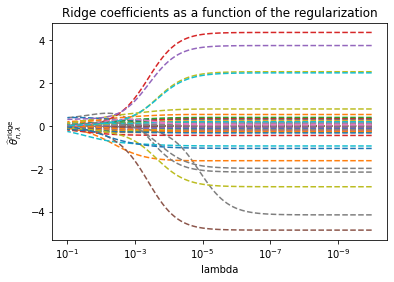
\includegraphics[width = .7\linewidth]{./Illustrations/ridge_coef.png}
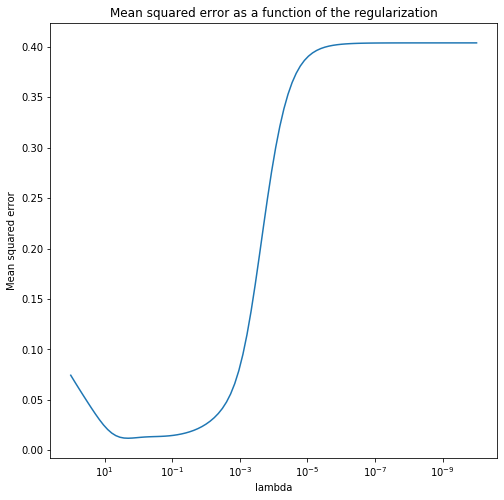
\includegraphics[width = .7\linewidth]{./Illustrations/ridge_rmse_test.png}
\end{center}
\caption{Ridge regression is used to predict the Brazilian inflation based on many observed variables, see \url{https://github.com/gabrielrvsc/HDeconometrics/}. The model is trained using $n=140$ data with for each $1\leqslant i \leqslant n$, $X_i\in\rset^{93}$, i.e. $d  =93$. The features are econometric data available each month. (Top) Estimated coefficient $\widehat \param^{\mathrm{ridge}}_{n,\lambda}$ as a function of $\lambda$. (Bottom) Mean squared error between the true observations and the predictions over the test set with $15$ new data points.}
\end{figure}


\begin{figure}
\begin{center}
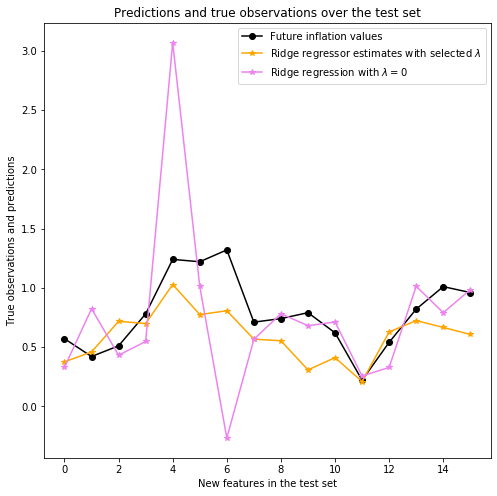
\includegraphics[width = .7\linewidth]{./Illustrations/ridge_pred_inflation.png}
\end{center}
\caption{Ridge regression is used to predict the Brazilian inflation based on many observed variables, see \url{https://github.com/gabrielrvsc/HDeconometrics/}. The model is trained using $n=140$ data with for each $1\leqslant i \leqslant n$, $X_i\in\rset^{93}$, i.e. $d  =93$. The features are econometric data available each month. In this experiment, 15 new data points in a test set are used to evaluate the Ridge estimator. We present an ordinary least squares estimate (i.e with $\lambda = 0$) and the estimate obtained by selecting $\lambda$ with a leave-one-out Cross-Validation. The MSE on the test set are 0.016 for the cross-validated $\lambda$ and 0.398 for $\lambda = 0$.}
\end{figure}



%%%%%%%%%%%%%%%%%%%%%%%%%%%%%%%%%%%%%
%%%%%%%%%%%%%%%%%%%%%%%%%%%%%%%%%%%%%
\section{Lasso regression}
The Least Absolute Shrinkage and Selection Operator (Lasso) regression is a $\mathrm{L}_1$ based regularized regression which aims at fostering sparsity. The objective is to solve the following minimization problem,
\begin{equation}
\label{eq:lasso:obj}
\widehat \param^{\mathrm{lasso}}_{\lambda,n}\in  \argmin_{\param\in\rset^d}  \left\{\frac{1}{n}\|Y - X\param\|_2^2 + \lambda\|\param\|_1\right\}\eqsp,
\end{equation}
where $\lambda>0$ and
\[
\|\param\|_1 = \sum_{j=1}^d|\param_j|\eqsp.
\]
The function $\param \mapsto n^{-1}\|Y - X\param\|_2^2 + \lambda\|\param\|_1$ is convex but not differentiable and the solution to this problem may  not be unique. 


\subsection{Computational issues}
A coordinate descent can be applied to solve the LASSO optimization problem. In this case, solving \eqref{eq:lasso:obj} amounts to producing iterative estimators, where at each iteration, a coordinate is selected to be updated. Then, the objective function  is optimized explicitly  with respect to the selected coordinate. For all $\param \in \rset^d$,  
\[
\nabla_\param \|Y - X\param\|_2^2 = - 2 X^\top (Y-X\param)\eqsp.
\]
Then, for all $1\leqslant j \leqslant d$, $(\nabla_\param \|Y - X\param\|_2^2)_j = -2 {\bf X}^\top_j (Y-X\param)$, where ${\bf X}_j$ is the $j$-th column of the matrix $X$. 
Define, for all $1\leqslant j \leqslant d$,
\[
\upsilon_{j}={\bf X}^\top_{j}\left(Y-\sum_{\substack{i=1\\ i\neq j}}^d\param_{i}{\bf X}_{i}\right)\eqsp.
\]
Assuming that the columns of $X$ are normalized, i.e. for all $1\leqslant k \leqslant d$, ${\bf X}^\top_{k}{\bf X}_{k}=1$, yields
\[
(\nabla_\param \|Y - X\param\|_2^2)_j = -2( \upsilon_j - \param_j)\eqsp.
\]
Consequently, for all $\param_j \neq 0$, 
\[
(\nabla_\param ( n^{-1}\|Y - X\param\|_2^2 +  \lambda\|\param\|_1))_j= \frac{2}{n}( \param_j - \upsilon_j + \lambda n\textrm{sign}(\param_j)/2)\eqsp.
\]
For all $1\leqslant j\leqslant d$,  $\param_j \mapsto  n^{-1}\|Y - X\param\|_2^2 + \lambda\|\param\|_1$ is convex and grows to infinity when $|\param_j|\to \infty$ and admits thus a minimum at some $\param_j^{\star}\in\rset$. 
\begin{enumerate}[-]
\item If $\param_j^{\star} \neq 0$, then
\[
\param_j^{\star} = \upsilon_j\left( 1 - \frac{\lambda n~\textrm{sign}(\param_j^{\star})}{2 \upsilon_j}\right)\eqsp,
\]
which yields, as  $\textrm{sign}(\param_j^{\star}) = \textrm{sign}(\upsilon_j)$,
\[
\param_j^{\star} = \upsilon_j\left(1 - \frac{\lambda n }{2 |\upsilon_j|}\right)
\]
and
\[
1 - \frac{\lambda n }{2 |\upsilon_j|} \geqslant 0\eqsp.
\]
\item If $1 - \lambda n/(2 |\upsilon_j|)<0$, there is no solution to $(\nabla_\param ( n^{-1}\|Y - X\param\|_2^2 +  \lambda\|\param\|_1))_j=0$ for $\param_j \neq 0$.  Since $\param_j \mapsto  n^{-1}\|Y - X\param\|_2^2 + \lambda\|\param\|_1$ admits a minimum, $\param_j^{\star}=0$. 
\end{enumerate}
Therefore,
\[
\param_j^{\star} = \upsilon_j\left( 1 - \frac{\lambda n}{2 |\upsilon_j|}\right)_+\eqsp.
\]
An algorithm to approximatively solve the Lasso regression problem proceeds as described in Algorithm~\ref{alg:lasso}.
\begin{algorithm}
\centering
\begin{algorithmic}
\State Choose randomly an initial estimate $\widehat \param_n^{(0)}\in\rset^d$.
\For{$p=1$ to $p = n_\mathrm{iter}$}
\State Choose randomly a coordinate $j\in\{1,\ldots, d\}$.
\State Compute
\[
\upsilon_{j}={\bf X}^\top_{j}\left(Y-\sum_{\substack{i=1\\ i\neq j}}^d\widehat\param^{(p-1)}_{n,i}{\bf X}_{i}\right)\eqsp.
\]
\State If $1 - \lambda n/(2 |\upsilon_j|)>0$, set 
\[
\widehat\param^{(p)}_{n,j}= \upsilon_j\left(1 - \frac{\lambda n }{2 |\upsilon_j|}\right)
\]
\State If $1 - \lambda n/(2 |\upsilon_j|)<0$, set $\widehat\param^{(p)}_{n,j}=0$.
\State For all $1\leqslant k \leqslant d$, $k\neq j$, set $\widehat\param^{(p)}_{n,k} = \widehat\param^{(p-1)}_{n,k}$.
\EndFor
\end{algorithmic}
\caption{Coordinate descent LASSO solver}
\label{alg:lasso}
\end{algorithm}

\subsection{Risk analysis of LASSO regression problem}
\begin{proposition}
Consider a well specified model where $\varepsilon \sim \mathcal{N}(0,\sigma_\star^2 I_n)$. Then, choosing $n\lambda_\star^2/(16\sigma_\star^2  \|\Sigma\|_\infty) = \log(dn)$ yields
$$
\frac{1}{n}\bE\left[\|X(\widehat\param^{\mathrm{lasso}}_{\lambda_\star,n}-\param_\star)\|_2^2\right] \leqslant  16\sigma_\star\sqrt{\frac{\log(dn)}{n}}\|\Sigma\|_\infty^{1/2}\|\param_\star\|_1  + 3\sqrt{2}\frac{\sigma_\star^2}{n\sqrt{d}} \eqsp.
$$
\end{proposition}

\begin{proof}
By definition of $\widehat\param^{\mathrm{lasso}}_{\lambda_\star,n}$, for all $\param\in\rset^d$,
$$
\frac{1}{n}\|Y - X\widehat\param^{\mathrm{lasso}}_{\lambda_\star,n}\|_2^2 + \lambda\|\widehat\param^{\mathrm{lasso}}_{\lambda_\star,n}\|_1 \leqslant \frac{1}{n}\|Y - X\param_\star\|_2^2 + \lambda\|\param_\star\|_1\eqsp.
$$
As $Y = X\param_\star + \varepsilon$, this yields
$$
\frac{1}{n}\|\varepsilon - X(\widehat\param^{\mathrm{lasso}}_{\lambda_\star,n}-\param_\star)\|_2^2 + \lambda\|\widehat\param^{\mathrm{lasso}}_{\lambda_\star,n}\|_1 \leqslant \frac{1}{n}\|\varepsilon\|_2^2 + \lambda\|\param_\star\|_1\eqsp.
$$
Therefore,
$$
\frac{1}{n}\|X(\widehat\param^{\mathrm{lasso}}_{\lambda_\star,n}-\param_\star)\|_2^2 + \lambda\|\widehat\param^{\mathrm{lasso}}_{\lambda_\star,n}\|_1 \leqslant \frac{2}{n}\varepsilon^\top X(\widehat\param^{\mathrm{lasso}}_{\lambda_\star,n}-\param_\star) + \lambda\|\param_\star\|_1\eqsp.
$$
and
\begin{align}
\|X(\widehat\param^{\mathrm{lasso}}_{\lambda_\star,n}-\param_\star)\|_2^2  &\leqslant 2\varepsilon^\top X(\widehat\param^{\mathrm{lasso}}_{\lambda_\star,n}-\param_\star) + \lambda n \|\param_\star\|_1 - \lambda n \|\widehat\param^{\mathrm{lasso}}_{\lambda_\star,n}\|_1\eqsp,\label{eq:lasso:general:bound}\\
&\leqslant 2 \|X^\top \varepsilon\|_\infty \|\widehat\param^{\mathrm{lasso}}_{\lambda_\star,n}-\param_\star\|_1   + \lambda n \|\param_\star\|_1 - \lambda n \|\widehat\param^{\mathrm{lasso}}_{\lambda_\star,n}\|_1\eqsp.\nonumber
\end{align}
On the other hand, writing $\Sigma = n^{-1}X^\top X$,
$$
\bP\left(\|X^\top\varepsilon\|_\infty \geqslant \frac{n\lambda}{2}\right) \leqslant \sum_{j=1}^{d} \bP\left(|X^\top\varepsilon|_j \geqslant \frac{n\lambda}{2}\right) \leqslant 2\sum_{j=1}^{d}\mathrm{exp}\left\{-n\lambda^2/(8\sigma_\star^2  \Sigma_{jj})\right\} \leqslant 2 d\mathrm{exp}\left\{-n\lambda^2/(8\sigma_\star^2  \|\Sigma\|_\infty\right\}\eqsp,
$$
as for all $1\leqslant j\leqslant d$, $X^\top\varepsilon\sim \mathcal{N}(0,\sigma_\star^2 X^\top X)$. Therefore, with probability at least $1 - 2 d\mathrm{exp}\left\{-n\lambda^2/(8\sigma_\star^2  \|\Sigma\|_\infty\right\}$,
$$
\|X(\widehat\param^{\mathrm{lasso}}_{\lambda_\star,n}-\param_\star)\|_2^2  \leqslant  \lambda n  \|\widehat\param^{\mathrm{lasso}}_{\lambda_\star,n}-\param_\star\|_1   + \lambda n \|\param_\star\|_1 - \lambda n \|\param^{\mathrm{lasso}}_{\lambda_\star,n}\|_1
$$
and
$$
\frac{1}{n}\|X(\widehat\param^{\mathrm{lasso}}_{\lambda_\star,n}-\param_\star)\|_2^2  \leqslant 2\lambda \|\param_\star\|_1 \eqsp.
$$
Let $A = \{\|X^\top\varepsilon\|_\infty < n\lambda / 2\}$. Then,
\begin{align*}
\bE\left[\|X(\widehat\param^{\mathrm{lasso}}_{\lambda_\star,n}-\param_\star)\|_2^2\right] \leqslant 2 n \lambda \|\param_\star\|_1 + \bE\left[\|X(\widehat\param^{\mathrm{lasso}}_{\lambda_\star,n}-\param_\star)\|_2^2 \1_{A^c}\right]\eqsp.
\end{align*}
Note that, by \eqref{eq:lasso:general:bound}, $\|X(\widehat\param^{\mathrm{lasso}}_{\lambda_\star,n}-\param_\star)\|_2^2 \leqslant 2 \|\varepsilon \|_2 \|X(\param^{\mathrm{lasso}}_{\lambda_\star,n}-\param_\star)\|_2 + \lambda n \|\param_\star\|_1 \leqslant  \|\varepsilon \|_2^2/2 +  \|X(\param^{\mathrm{lasso}}_{\lambda_\star,n}-\param_\star)\|_2^2/2 + \lambda n \|\param_\star\|_1$. Then,
$$
\bE\left[\|X(\widehat\param^{\mathrm{lasso}}_{\lambda_\star,n}-\param_\star)\|_2^2\right] \leqslant 2 n \lambda \|\param_\star\|_1 + \bE\left[ (\|\varepsilon \|_2^2 + 2\lambda n \|\param_\star\|_1) \1_{A^c}\right]
$$
and by Cauchy-Schwarz inequality,
$$
\bE\left[\|X(\widehat\param^{\mathrm{lasso}}_{\lambda_\star,n}-\param_\star)\|_2^2\right] \leqslant 4 n \lambda \|\param_\star\|_1 + \bE\left[\|\varepsilon \|_2^4\right]^{1/2} \bP\left(A^c\right)^{1/2}\eqsp.
$$
Using that $\bE[\|\varepsilon \|_2^4]^{1/2}\leqslant 3n\sigma_\star^2$ yields
$$
\frac{1}{n}\bE\left[\|X(\widehat\param^{\mathrm{lasso}}_{\lambda_\star,n}-\param_\star)\|_2^2\right] \leqslant  4\lambda \|\param_\star\|_1  + 3\sigma_\star^2 \cdot \sqrt{2 d}\mathrm{exp}\left\{-n\lambda^2/(16\sigma_\star^2  \|\Sigma\|_\infty\right\}\eqsp.
$$
By choosing $\lambda$ so that $n\lambda^2/(16\sigma_\star^2  \|\Sigma\|_\infty) = \log(dn)$, we obtain
$$
\frac{1}{n}\bE\left[\|X(\widehat\param^{\mathrm{lasso}}_{\lambda_\star,n}-\param_\star)\|_2^2\right] \leqslant  16\sigma_\star\sqrt{\frac{\log(dn)}{n}}\|\Sigma\|_\infty^{1/2}\|\param_\star\|_1  + 3\sqrt{2}\frac{\sigma_\star^2}{n\sqrt{d}} \eqsp.
$$
\end{proof}
